

\section{Context-Sensitive Grammars}\fbeg{}\begin{frame}{\ft{Rules and Contexts in Parsing Code}}


%\doubleFrame{Contexts and flags}

\hspace*{-17pt}\begin{tikzpicture}

\node[anchor=south west,inner sep=0] (image) at (0,0){%

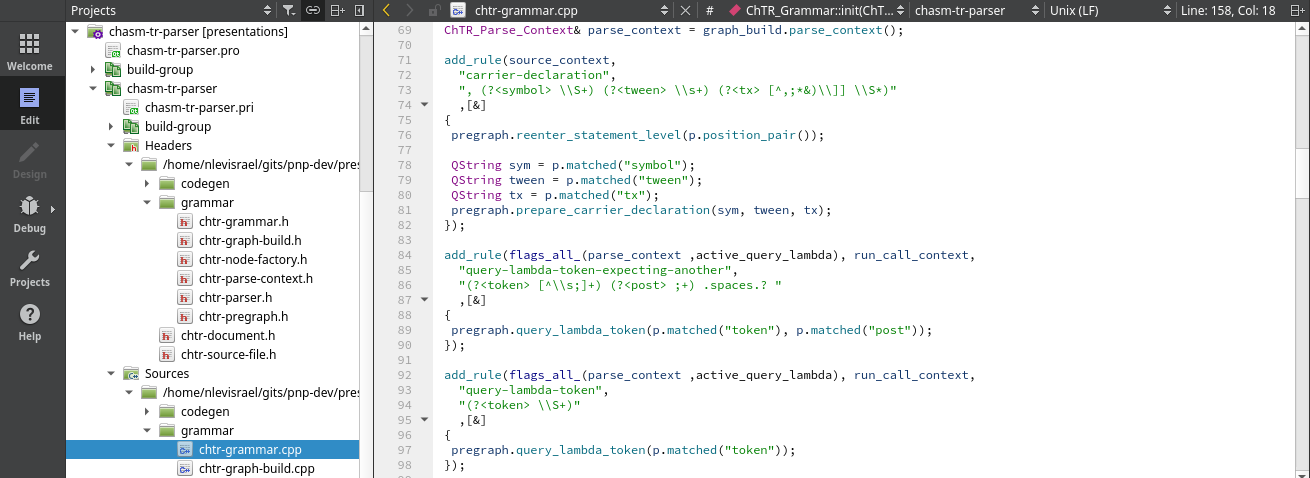
\includegraphics[width=34cm, clip, trim={180pt 0 0 0}]{ss/ss-parser.png}

};

\ann{BlueGreen!30!red}{1}{.8mm}{blue!50!orange}{0.5}{11.2,12.6}{3.2}{.45}{.7}

 \node [anchor=west,fill=blue!50!orange,opacity=0.5, text opacity=1, inner sep=3, text width=5cm]
  (longnote) at (2.7,12) {\vspace{-9pt} %  %{\color{rb!85!red}{
  {\cframedboxc{BlueGreen!30!red}{\large \textbf{\q{Outer} contexts can be grouped such that one triggers another}}}};


\ann{brown!70!red}{1}{.6mm}{purple!50!cyan}{0.5}{12.86,5.82}{6.9}{.45}{.85}

 \node [anchor=west,fill=purple!50!cyan,opacity=0.5, text opacity=1,inner sep=3, text width=6cm]
  (longnote) at (17.3,7.2) {\vspace{-8pt} %  %{\color{rb!85!red}{
  {\cframedboxc{brown!70!red}{\large \textbf{Rules are regular-expression strings plus callbacks}}}};



\ann{BlueGreen!10!magenta}{1}{.5mm}{red!50!orange}{0.3}{14,.83}{8}{.45}{.9}

 \node [anchor=west,fill=red!50!orange,opacity=0.5, text opacity=1,inner sep=3, text width=9cm]
  (longnote) at (13.2,1.9) {\vspace{-8pt} %  %{\color{rb!85!red}{
  {\cframedboxc{BlueGreen!10!magenta}{\large \textbf{\q{Inner} contexts are combinable boolean flags}}}};


% \node [anchor=west,fill=brown!20!white,inner sep=7, text width=14cm]
%  (longnote) at (5.5,7) {\vspace{-8pt}%  %{\color{rb!85!red}{
%  {\cframedbox{\large \textbf{...}}}};

\end{tikzpicture}


\end{frame}


